\documentclass[12pt]{report}

\usepackage[a4paper]{geometry}
%\geometry{left=2.5cm,right=2.5cm,top=2.5cm,bottom=2.5cm, a4paper}
\usepackage[utf8]{inputenc}
\usepackage{amsmath}
\usepackage{amsthm}
\usepackage{amssymb}
\usepackage{ulem}
\usepackage{graphicx}
\usepackage{caption}
\graphicspath{}
\usepackage[document]{ragged2e}
\usepackage{setspace}
\usepackage{tabularx}
\usepackage[slovene]{babel}
\usepackage{textcomp, gensymb}
\usepackage{siunitx}
\usepackage{pdfrender,xcolor}
\usepackage{hyperref}
\usepackage{xurl}
\usepackage{float}
\usepackage{titlesec}

\newfloat{slika}{htbp}{loc}
\floatname{slika}{Slika}

\newfloat{tabela}{htbp}{loc}
\floatname{tabela}{Tabela}

% Differential
\newcommand{\diff}{\mathrm{d}}

\title{
  
\includegraphics[width=0.4\textwidth]{fmf_logo}\\
  {\small Oddelek za fiziko} \\
  {Določanje Boltzmannove konstante $k_B$}\\
  {\small Poročilo pri fizikalnem praktikumu IV}\\

}
\date{}
\author{ Kristofer Č. Povšič \\[5 cm]
 \small  Asistentka: Jelena Vesić
}


\titleformat{\chapter}[hang]{\Huge\bfseries}{\thechapter{. }}{0pt}{\Huge\bfseries}

\setlength\parindent{0pt}

\begin{document}

\setcounter{page}{2}

\maketitle

\chapter*{Uvod}

Boltzmannovo konstanto $k_B$ lahko izmerimo preko tokov znotraj bipolarnega tranzistorja. Tranzistor ima tri kontakte emitor, kolektor in bazo. Slednja dva v vaji sklenemo, da pride do kratkega stika in merimo odvisnost toka skozi kolektor. Napoved te odvisnosti je podana z Ebers-Millovo enačbo:

\begin{equation}
  I_C = I_S(T)\left[exp\left(\frac{e_0 U_{BE}{k_B T}}\right) - 1\right]
\end{equation}

kjer so $e_0$ osnovni naboj, $T$ absolutna temperatura, $U_{BE}$ pozitivna napetost med bazo in emitorjem ter $I_S (T)$ velikost nasičenega toka v zaporni smeri. Brez izgube natančnosti lahko poenostavimo v 

\begin{equation}
  I_C \approx I_S(T) exp\left(\frac{e_0 U_{BE}}{k_B T}\right)
\end{equation}


\chapter*{Naloga}

\begin{enumerate}
  \item Izmerite kolektorski tok tranzistorja $I_C$ v odvisnosti od $U_{BE}$ pri treh temperaturah: približno $15 ^\circ C$, $35 ^\circ C$, $55 ^\circ C$
  \item Določite razmerje $\frac{e_0}{k_B}$
  \item Izmerite temperaturno odvisnost kolektorskega toka tranzistorja pri dveh napetostih $U_{BE}$ približno $0.5V$ in $0.58V$
\end{enumerate}


\begingroup
\let\clearpage\relax

\chapter*{Potrebščine}

\begin{itemize}
  \item bipolarni \verb+n-p-n+ tranzistor tipa BC182B
  \item potenciometer in baterija ali drug stabilen vir enosmerne napetosi do 1.5V
  \item voltmeter(Voltcraft 870), namizni multimeter (SigLent SDM 3060X)
  \item žice
  \item termometer, Dewarjeva posoda in čaše za vodo 
  \item prenosnik s programom \verb+Boltz+ 
\end{itemize}

\chapter*{Navodilo}

Vpišem se v računalnik in zaženem program \verb+Boltz+. Vključim multimetre in jih povežem z računalnikom. Za prvi del vodo segrejem na tri različne temperature $15 ^\circ C$, $35 ^\circ C$, $55 ^\circ C$ in vsakič potopim tranzistor v vodo ter spreminjam napetost na potenciometru od $0.4V$ do $0.6V$. Potem narišem diagram $\ln (I_C/ I)$ v odvisnosti od $U_{BE}$, ki naj bi bil v teoriji premica z naklonom $e_0/k_B T$. 

Za drugi del nastavim potenciometer na eno izmed dveh, v nalogi omenjenih vrednosti, in s potopljenim tranzistorjem segrevam vodo od ledišča do vrelišča in beležim, kako se tok spreminja v odvisnosti od temperature. 

\endgroup


\chapter*{Obdelava podatkov}

Za prvi del dobim sledeč graf: 

\begin{slika}
  \centering
  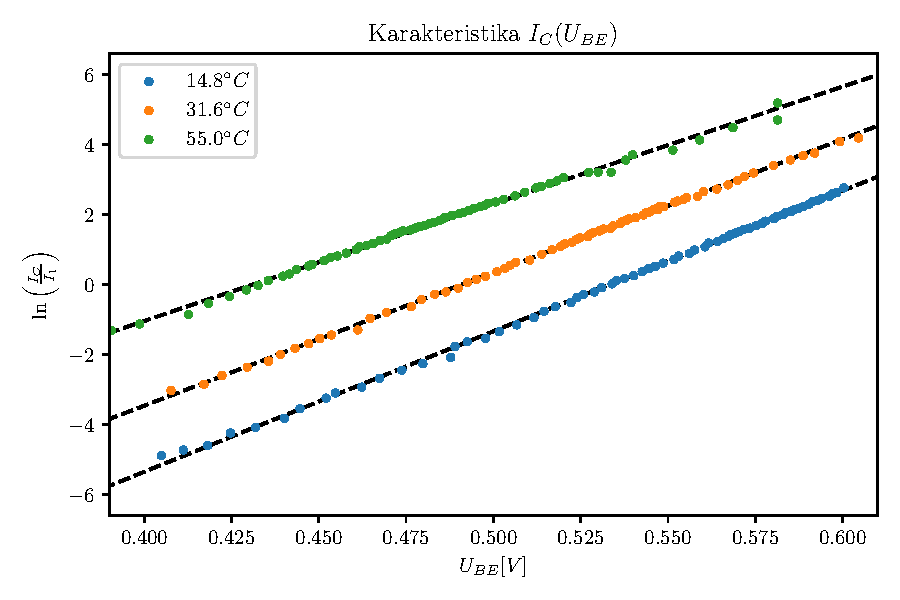
\includegraphics{1graf}
  \caption{\small Graf prikazuje odvisnost kolektorskega toka od napetosti med bazo in emitorjem pri treh različnih temperaturah v legendi. Črtkane črte so regresivne premice podatkov.}
\end{slika}

\begin{tabela}
  \centering
  \[
  \begin{array}{|c|c|c|}\hline
    T[^\circ C] & \frac{e_0}{k_B} [\cdot 10^{-6} \frac{V}{K}] & k_B [\cdot 10^{-23} \frac{J}{K}] \\ \hline 
    287.9 \pm 0.4 & 86.4 \pm 0.3 & 1.38 \pm 0.05 \\ \hline
    304 \pm 1 & 86.1 \pm 0.4 & 1.38 \pm 0.06 \\ \hline
    328 \pm 1.6 & 91.0 \pm 0.8 & 1.4 \pm 0.1 \\ \hline
  \end{array}
  \]
\end{tabela}

Za drugi del dobim naslednji graf: 

\begin{slika}
  \centering
  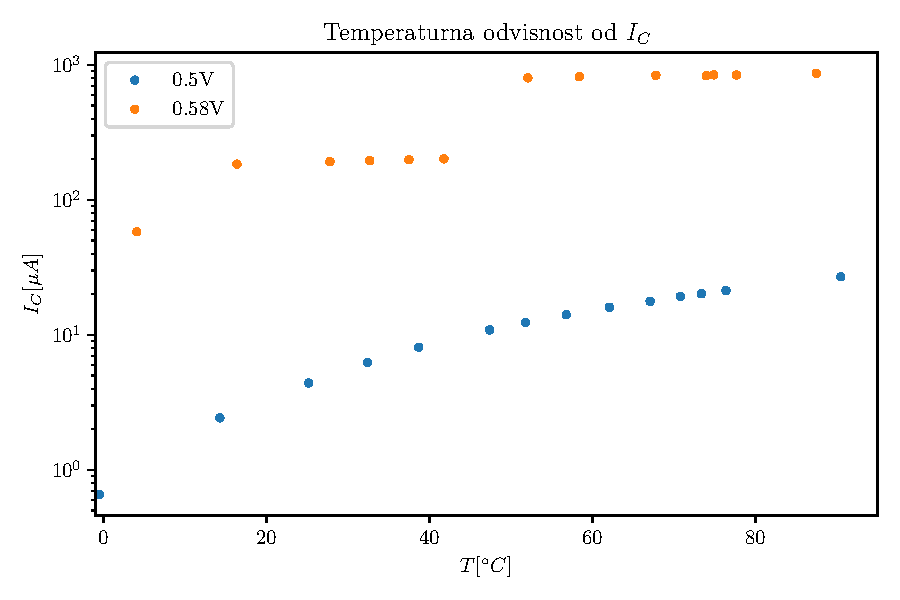
\includegraphics{2graf}
  \caption{\small Odvisnost kolektorskega toka od temperature pri dveh različnih napetostih med bazo in emitorjem. Pri napetosti $0.58V$ za nizke in visoke temperature izmerki očitno izstopajo.}
\end{slika}


\end{document}